
\section*{Ejercicio 2}
\subsection{Análisis teórico}
El circuito a analizar consiste, a grandes rasgos, en un amplificador no inversor.
Para su estudio teórico se tomarán dos modelos, donde, en primer lugar, se considerará al amplificador operacional en su versión ideal, para luego introducir no idealidades en su impedancia de entrada, salida y en la ganancia del mismo.
Los valores de las resistencias a utilizar fueron reemplazados por su valor comercial más cercano, resultando en que el circuito a analizar sea el de la figura \ref{fig:initial_circuit}.
\begin{figure}[H]
    \begin{minipage}{\textwidth}
        \centering
        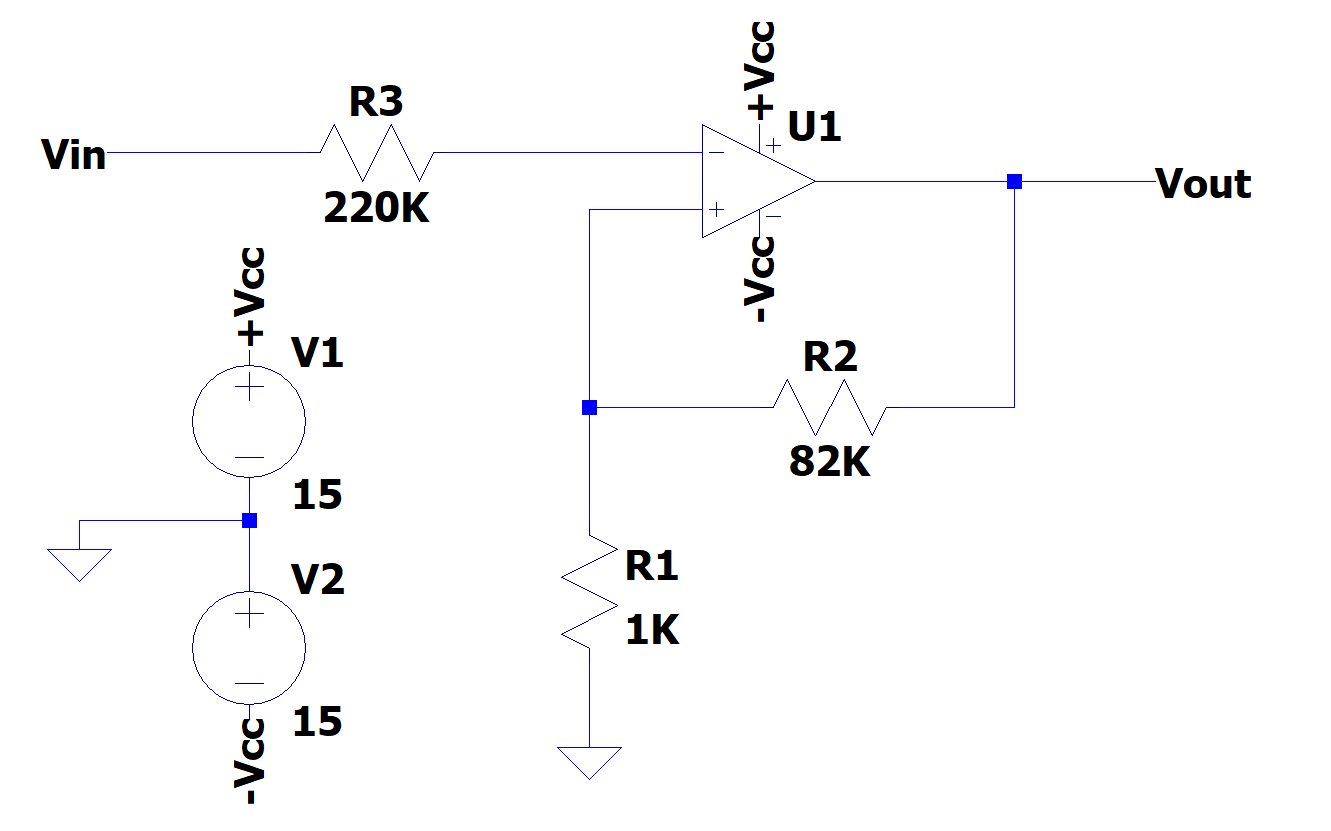
\includegraphics[width=\textwidth]{../EJ2/recursos_para_el_informe/circuito_a_analizar_ideal}
        \caption{Circuito a analizar.}
        \label{fig:initial_circuit}
    \end{minipage}\hfill
\end{figure}

Ha de prestarse especial atención al nodo de la entrada no inversora del operacional.
El mismo se encuentra a alta impedancia, ya que a su izquierda tiene la resistencia de $220K\Omega$, y a su derecha la impedancia interna del operacional (también alta).
Esto lo convierte esencialmente en una antena, susceptible a captar señales de su entorno y, dado que está conectado a un circuito con una alta amplificación (cercana a los 40dB), amplificar esta señal parásita a la salida.\par
Este problema fue afrontado al realizar las mediciones con el operacional LM833 (uno de los dos pedidos), y se ofreció una solución al mismo que será detallada más adelante en las conclusiones del ejercicio.
Luego, para el segundo operacional (NE5534), se decidió reemplazar a la misma por una de inferior valor, y se tomó como criterio hacer uso de la resistencia óptima para la compensación de las corrientes de bias.
El valor para tal resistencia se obtiene de tomar el paralelo entre la resistencia de entrada al sistema, y la de feedback:
\begin{equation}
    R_3' = \frac{R_1 \cdot R_2}{R_1 + R_2} = \frac{1K\Omega \cdot 82K\Omega}{1K\Omega + 82K\Omega} \approx 1K\Omega
\end{equation}

\subsubsection{Modelo ideal}
La primer aproximación al comportamiento del circuito se realizará considerando al amplificador operacional como un componente ideal, es decir, $Av = \inf$, $Z_{in_{opamp}} = \inf$, $Z_{out_{opamp}} = 0$.
De esta manera, sin importar el modelo de operacional utilizado, se tiene que:
\begin{equation}
    \label{eq:ideal_gain}
    \frac{v_{out}}{v_{in}} = 1 + \frac{R_2}{R_1} = 1 + \frac{82 K\Omega}{1 K\Omega} = 83 \implies 38,38 dB
\end{equation}

Se desprende también, de las condiciones de idealidad impuestas, que la impedancia de entrada del circuito será infinita.


\subsubsection{Modelo con impedancia de entrada, salida, y ganancia finita}
Para la resolución del circuito con las consideraciones ya mencionadas, es necesario ahora especificar qué datos serán utilizados para los cálculos.
Los mismos fueron obtenidos de las correspondientes datasheets 
\footnote{Datasheet para operacional LM833: https://www.ti.com/lit/ds/symlink/lm833.pdf \\Datasheet para operacional NE5534: https://www.onsemi.com/pub/Collateral/NE5534-D.PDF}, 
y se presentan en el cuadro \ref{tab:parameters_for_equations}.
\begin{table}[H]
    \label{tab:parameters_for_equations}
    \centering
    \begin{tabular}{|l|lllll|}
        \hline
        \textbf{\begin{tabular}[c]{@{}l@{}}Modelo de operacional\end{tabular}} & \textbf{\begin{tabular}[c]{@{}l@{}}$f_0$ (Hz)\end{tabular}} & \textbf{\begin{tabular}[c]{@{}l@{}}$A_0$ \end{tabular}} & \textbf{$r_{in_{opamp}}(K\Omega)$} & \textbf{$r_{out_{opamp}}(\Omega)$} & \textbf{$C_{in_{opamp}}(pF)$} \\ \hline
        \textbf{LM833}                                                         & $16 \cdot 10^3$                                             & $1000$                                                  & $175$                              & $37$                               & $12$                          \\
        \textbf{NE5534}                                                        & $100$                                                       & $10 \cdot 10^5$                                         & $100$                              & $0,3$                              & -                             \\ \hline
        \end{tabular}
    \caption{Parámetros para cálculo de circuito no ideal.}
\end{table}

Se modelizará al operacional mediante el circuito \ref{fig:non_ideal_circuit}.
\begin{figure}[H]
    \begin{minipage}{\textwidth}
        \centering
        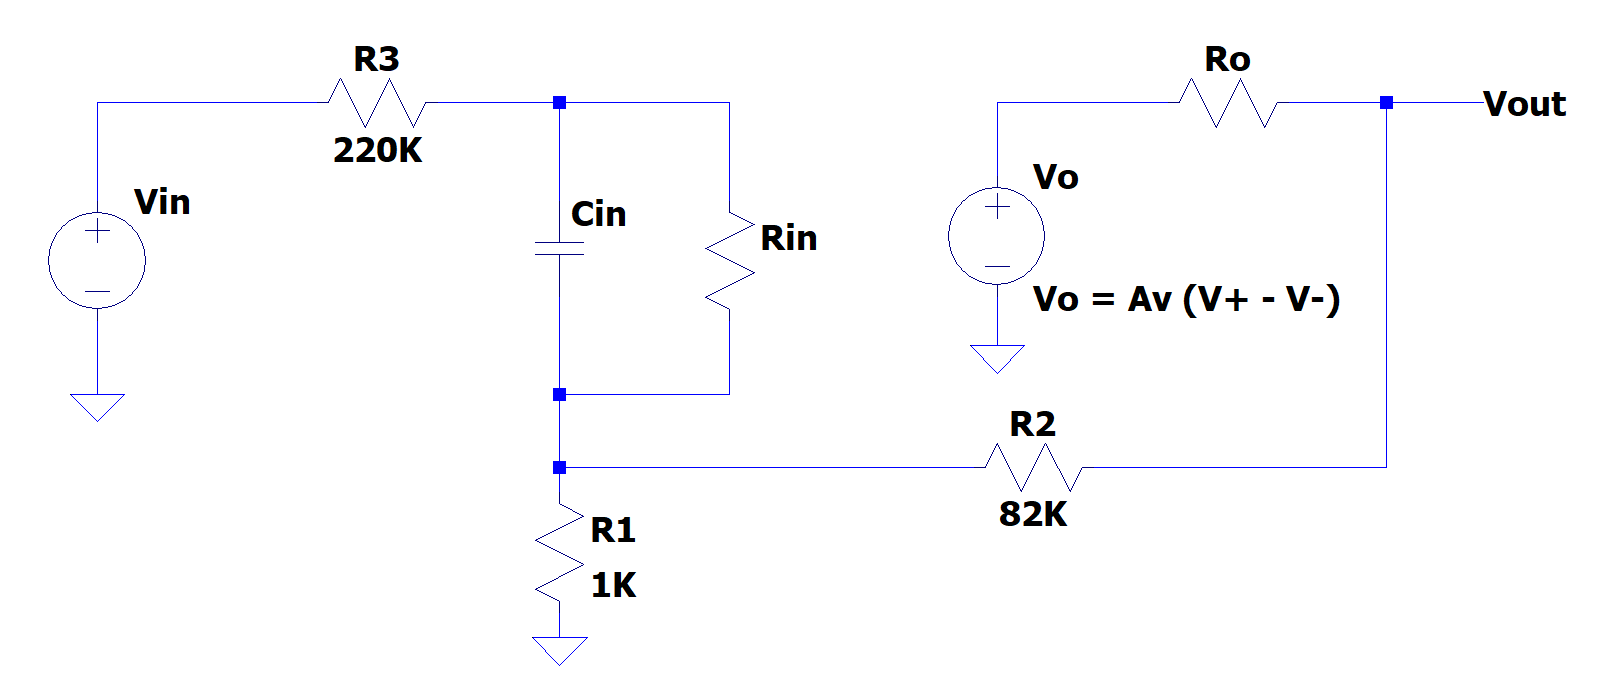
\includegraphics[width=\textwidth]{../EJ2/recursos_para_el_informe/circuito_a_analizar_no_ideal}
        \caption{Circuito a analizar.}
        \label{fig:non_ideal_circuit}
    \end{minipage}\hfill
\end{figure}

Se entiende al circuito como dos mallas cuyas ecuaciones son las descriptas en \ref{eq:system_meshes}, que se extraen del circuito \ref{fig:meshes_circuit}.
\begin{figure}[H]
    \begin{minipage}{\textwidth}
        \centering
        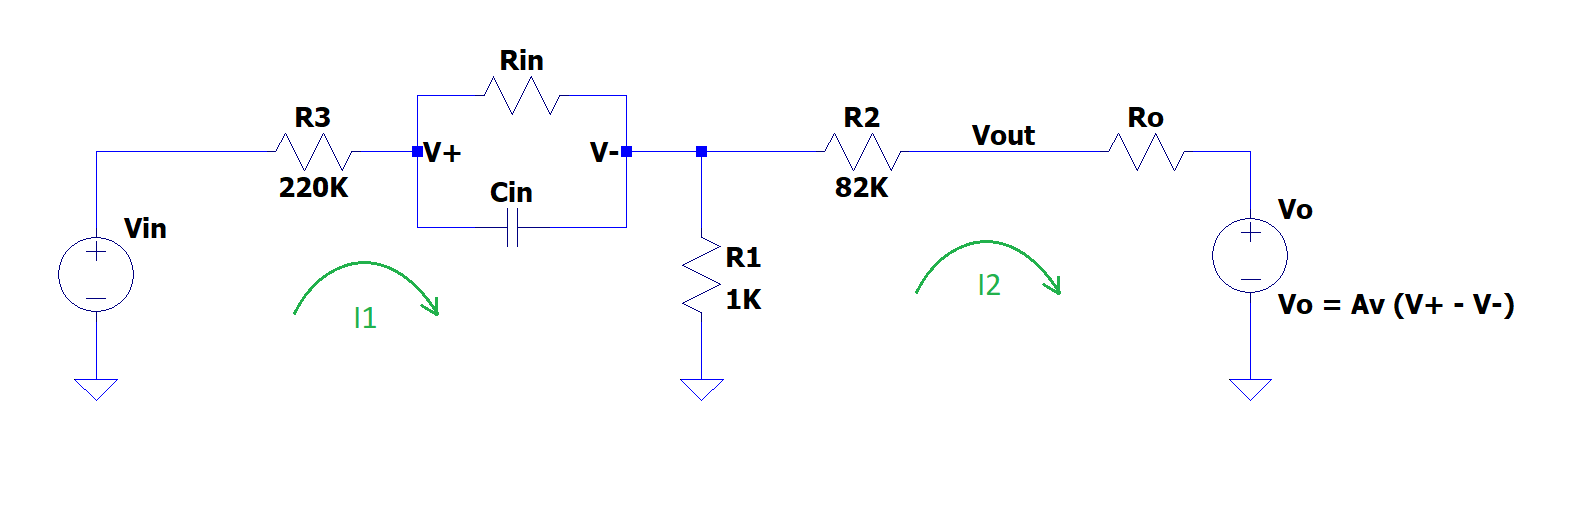
\includegraphics[width=\textwidth]{../EJ2/recursos_para_el_informe/circuito_mallas}
        \caption{Circuito a analizar.}
        \label{fig:meshes_circuit}
    \end{minipage}\hfill
\end{figure}

\begin{align}
    \label{eq:system_meshes}
    &v_{in} - i_1 \cdot R_3 - i_1 \cdot Z_{in} - \left(i_1 - i_2\right) \cdot R_1 = 0 \\
    &-\left(i_2 - i_1\right) \cdot R_1 - i_2 \cdot R_2 - I_2 \cdot R_0 - v_o = 0 \\
    &v_o = \left(v^+ - v^-\right) \cdot A_v \\
    &v^+ = v_{in} - i_1 \cdot R_3 \\
    &v^- = v_{in} - i_1 \cdot R_3 - i_1 \cdot Z_{in} \\
    &Z_{in} = \frac{R_{in}}{R_{in} \cdot C_{in} \cdot s + 1} \label{eq:zin} \\
    &A_v = \frac{A_0}{1+\frac{s}{\omega_p}}
\end{align}

Resolviendo para $i_2$ se obtiene que:
\begin{equation}
    i_2 = v_{in} \cdot \frac{R_1 - A_v \cdot Z_{in}}{R1 \cdot \left(A_v \cdot Z_{in} - R_1\right) + \left(R_3 + Z_{in} + R_1\right) \cdot \left(R_1 + R_2 + R_o\right)}
    \label{eq:i2}
\end{equation}

Y luego se expresan $v_{out}$ e $i_1$ en función de $i_2$ como:
\begin{align}
    \label{eq:i1_and_vout}
    &i_1 = \frac{v_{in} + i_2 \cdot R_1}{R_3 + Z_{in} + R_1} \\
    &v_{out} = v_{in} \cdot \frac{R_1}{R_3 + Z_{in} + R_1} + i_2 \cdot \frac{R_1^2}{R_3 + Z_{in} + R_1} + i_2 \cdot R_1 - i_2 \cdot R_2
\end{align}

\subsubsection{Ecuaciones teóricas para el LM833}
De los resultados obtenidos en \ref{eq:i1_and_vout}, y con los datos de la tabla \ref{tab:parameters_for_equations}, se tiene:
\begin{align}
    & \frac{v_{out}^{LM833}}{v_{in}} = \frac{1,11 \cdot 10^{-4} \cdot s^{4} + 1,105 \cdot 10^{3} \cdot s^{3} + 3,698 \cdot 10^{13} \cdot s^{2} + 3,471b\cdot 10^{20} \cdot s + 2,692 \cdot 10^{26}}
    {s^{4} + 1,034 \cdot 10^{7} s^{3} + 1,678 \cdot 10^{13} \cdot s^{2} + 1,203 \cdot 10^{19} s + 3,948 \cdot 10^{24}} \label{eq:LM833_transfer_fun} \\
    & Z_{in}^{LM833} = \label{eq:LM833_in_impedance} \\
\end{align}
\todo[inline]{NE5534 Transfer function}

\subsubsection{Ecuaciones teóricas para el NE5534}
De los resultados obtenidos en \ref{eq:i1_and_vout}, y con los datos de la tabla \ref{tab:parameters_for_equations}, se tiene:
\begin{align}
    & \frac{v_{out}^{NE5534}}{v_{in}} = \label{eq:NE5534_transfer_fun} \\
    & Z_{in}^{NE5534} = \label{eq:NE5534_in_impedance}
\end{align}
\todo[inline]{LM833 Input inpedance}
\todo[inline]{NE5534 Input inpedance}


\subsection{Simulación}
Para el análisis de los circuitos mediante herramientas de simulación se empleó el programa LTspice, para el cual se realizaron dos esquemáticos, uno para cada uno de los operacionales.
En ambos casos, se simuló la respuesta en frecuencia utilizando la función AC Analysis, y se obtuvieron así los diagramas de bode e impedancia de entrada del sistema, seleccionando las variables pertinentes a observar en el graficador.
A continuación se presentan los circuitos utilizados para tal fin:
\missingfigure{Circuit in LTspice for LM833}
\missingfigure{Circuit in LTspice for NE5534}